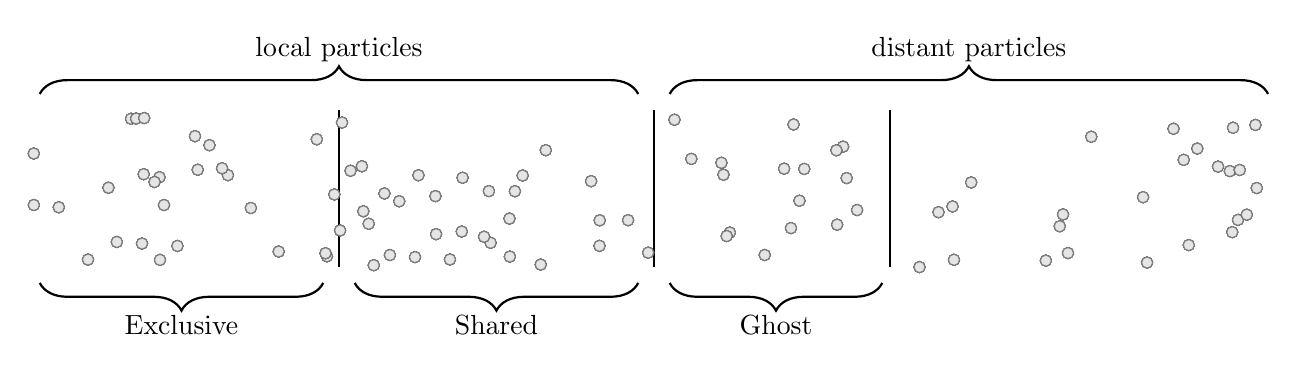
\begin{tikzpicture}
\pgfmathsetseed{1}
\def\nrand{100}
% braces on top : local; distant
\draw [thick,decorate,decoration={brace,amplitude=10pt}]
(0.2,2.2) -- (7.8,2.2) node [midway,above,yshift=8pt] 
{local particles};
\draw [thick,decorate,decoration={brace,amplitude=10pt}]
(8.2,2.2) -- (15.8,2.2) node [midway,above,yshift=8pt] 
{distant particles};

\draw [thick,decorate,decoration={brace,amplitude=10pt}]
 (3.8,-.2) -- (0.2,-.2) node [midway,below,yshift=-8pt] 
{Exclusive};
\draw [thick,decorate,decoration={brace,amplitude=10pt}]
(7.8,-.2) -- (4.2,-.2) node [midway,below,yshift=-8pt] 
{Shared};
\draw [thick,decorate,decoration={brace,amplitude=10pt}]
(10.9,-.2) -- (8.2,-.2) node [midway,below,yshift=-8pt] 
{Ghost};

% Vertical bars 
\draw[thick] (4,0) -- (4,2) node (exclusive) {};
\draw[thick] (8,0) -- (8,2) node (shared) {};
\draw[thick] (11,0) -- (11,2) node (ghosts) {};

\foreach \i in {1,2,...,\nrand}{
	\pgfmathsetmacro{\x}{((rand)+1)*8}
	\pgfmathsetmacro{\y}{((rand)+1)*1}
	\ifthenelse{ \lengthtest{\x cm < 4 cm}}
		{\draw[black!70,fill=red!90] (\x,\y) circle (2pt);}
		{\ifthenelse { \lengthtest{\x cm < 8 cm}}
			{\draw[black!70,fill=blue!90] (\x,\y) circle (2pt);}
			{\ifthenelse { \lengthtest{ \x cm < 11 cm }}
				{\draw[black!70,fill=black!30!green] (\x,\y) circle (2pt);}
				{\draw[black!50,fill=black!10] (\x,\y) circle (2pt);} 
			}
		}
}
\end{tikzpicture}